
%Not really sure what this pdf is, but I like it, and will post the link so I don't forget about it https://spie.org/samples/TT69.pdf
\section{Fluorescent Confocal Microscopy} \label{ch:microscopy}
Confocal Microscopy is a technique capable of probing a sample with true 3-Dimensional optical resolution. The technique works by only allowing in focus light through a pinhole. By changing the plane of focus, one can traverse an object azimuthally or reconstruct a full three-dimensional image by compiling a ``stack'' of these images.  

\begin{figure}[h!]
	\centering
	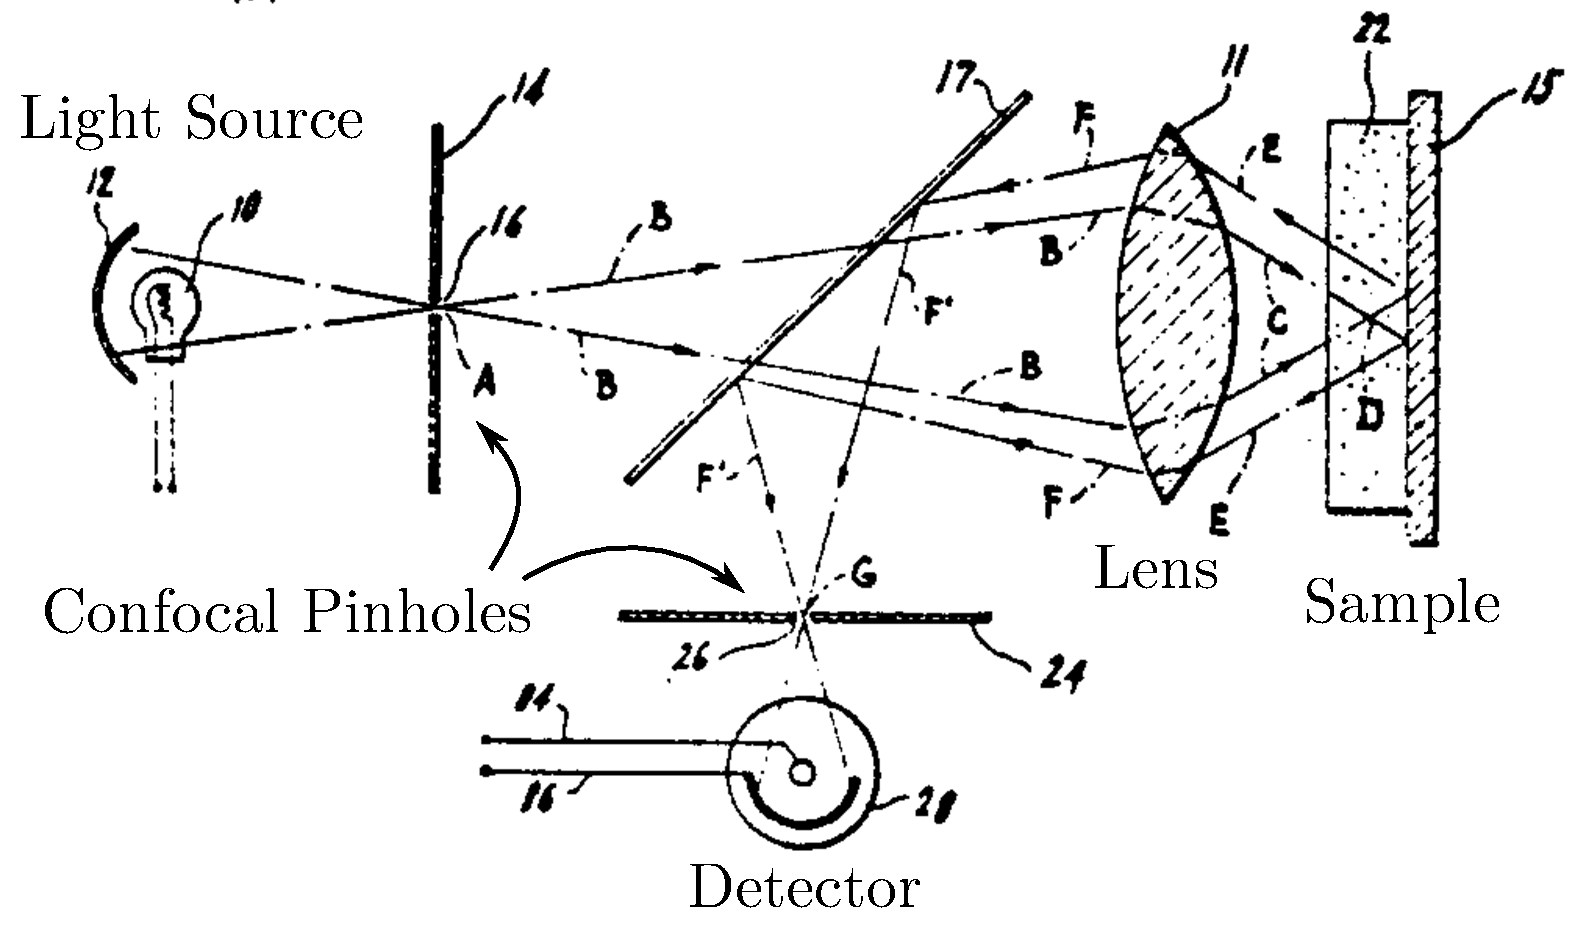
\includegraphics[width=\linewidth]{confocal_stuff/confocalpatent_crop2}
	\caption[Minsky Patent Diagram]{Above is a diagram from Marvin Minky's 1961 patent \cite{patent:3013467} for a confocal microscope. A pinhole before the photodetector blocks the out of plane light.}
	\label{fig:confocalpatent}
\end{figure}


\begin{wrapfigure}{r}{.6\textwidth}
	
	\centering
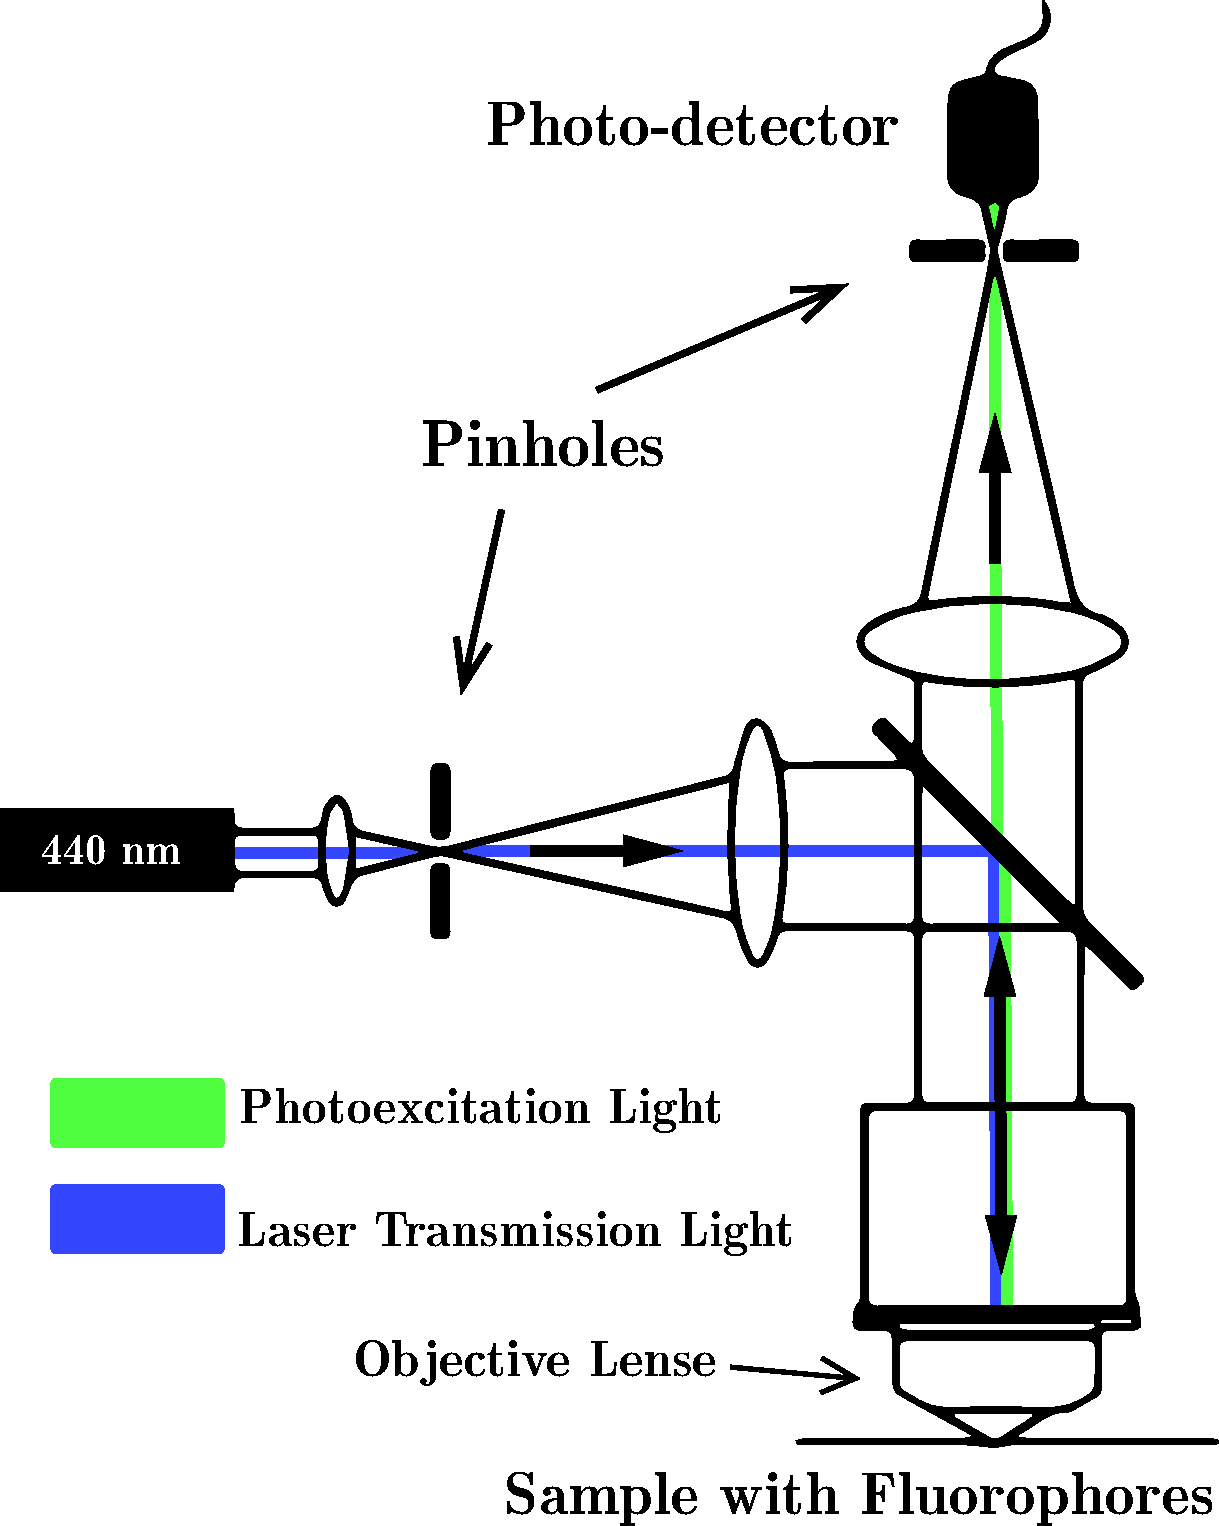
\includegraphics[width=\linewidth]{Chapters/Figures/confocal_fluorescent_diagram_b}
\caption[Fluorescent Confocal Microscopy]{In fluorescent confocal microscopy, a diachroic mirror is used to separate the laser light from that emitted by the excited fluorophores. }
\label{fig:confocalfluorescentdiagram}
	
	
\end{wrapfigure}
	
Fluorescent Confocal Microscopy works by the same general principle, only with the added complexity of optically-excitable fluorophores. These fluorophores absorb light from a narrow range of frequencies and re-emit fluorescent light at different and narrow frequency which can then be measured. This allows for a greater resolution to larger objects, as well as the ability to detect features that would otherwise be invisible to the microscope.  

Fluorescent Confocal Microscopy works by illuminating the specimen with a laser. The laser light passes through a pinhole, then is reflected by the dichroic mirror and then focused by the objective lens on a small area of the specimen. The re-emitted light from the fluorophores (photoexcitation) has a longer wavelength than the laser light, so only it is transmitted through mirror. The photoexcitation light then passes through the pinhole where it is travels to the photodetector. The net result of the process is a the measurement of photo-excitation light from a single plane of the probed sample. A diagram of this process can be found in figure \ref{fig:confocalfluorescentdiagram}.
%\begin{figure}[h!]
%	\centering
%	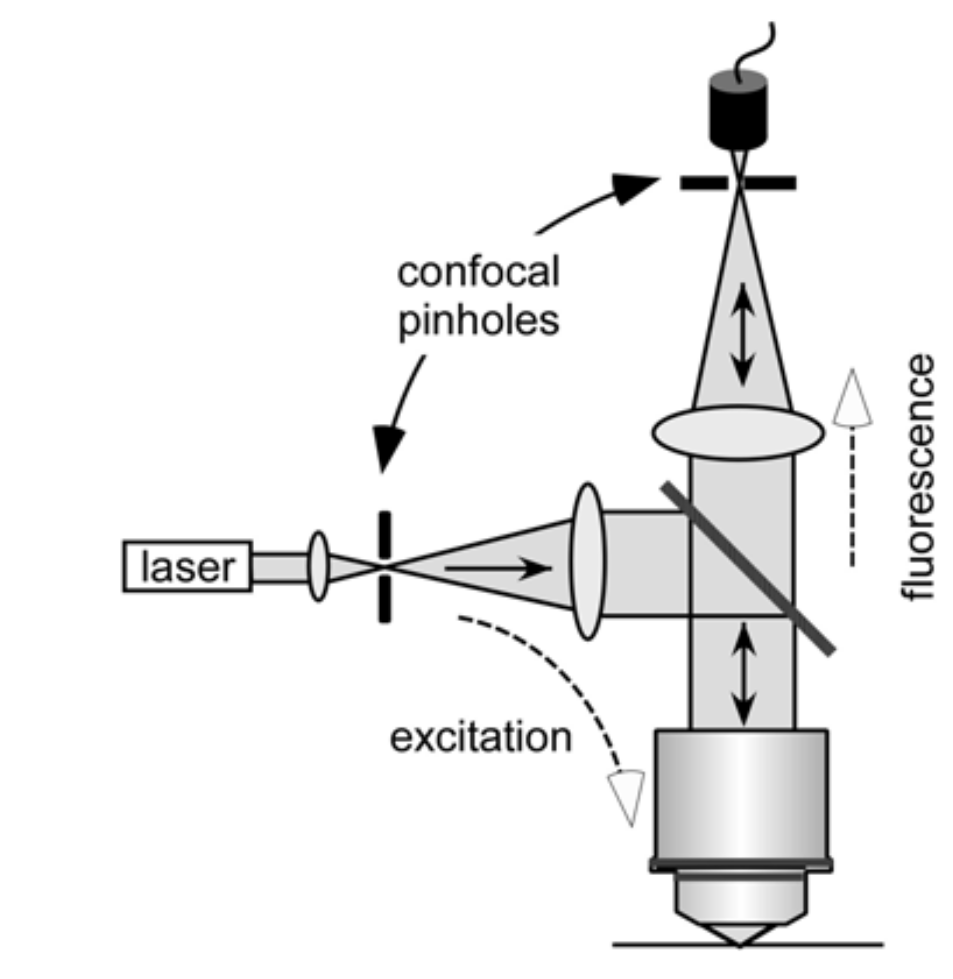
\includegraphics[width=.7\linewidth]{Chapters/Figures/confocal_fluorescent_diagram}
%	\caption[Fluorescent Confocal Microscopy]{In fluorescent confocal microscopy, a diachroic mirror is used to separate the laser light from that emitted by the excited fluorophores. }
%	\label{fig:confocalfluorescentdiagram}
%\end{figure}

\section{Applying Fluorescent Confocal Microscopy to the Sample}
In order to see our substrate with fluorescent confocal microscopy, we need to coat the surface of our substrate with tiny fluorescent beads (fluorophores) on the order of 40nm in radius. The detection of these fluorescent beads allows us to see the outline of the substrate's surface, as well as the indenting sphere, which displaces the beads beneath it as in sinks into the substrate. Directions for preparing a fluorescent bead solution in a borate buffer can be found in Appendix section \ref{appendix_beads}. 

\subsubsection{Fluorescent Confocal Microscopy Data Collection}
Data was obtained using the Nikon A1R HD25 Confocal Microscope. To take image stacks of the Fluorescent beads, we use a 60x water-immersion objective lens with a numerical aperture of 1.2. We set the laser to 440nm and adjust the power and gain (HV) as needed. Generally these values are around 5.0\% and 40 Volts, respectively. In order to get clear locating, it is important not to saturate the photo-detector. 

\begin{figure}
	\centering
	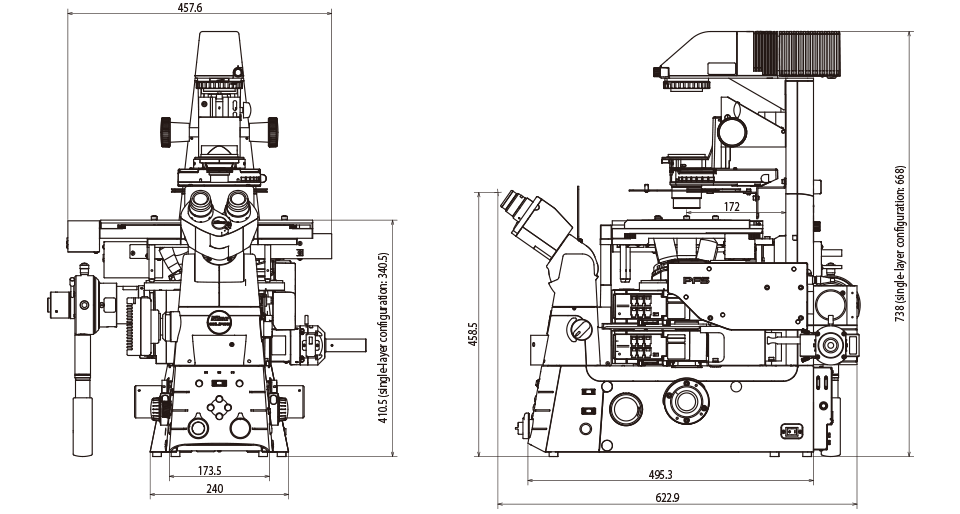
\includegraphics[width=0.8\linewidth]{confocal_stuff/Ti2_diagram_1}
	\caption[Nikon Ti2 Microscope Base]{The Nikon A1 Confocal Base}\todo[color=pink,inline]{Include the example setup image and cite the manual!}
	\label{fig:ti2diagram1}
\end{figure}

For silica spheres ranging from $5-50$ $\mu$m in size, we have found the best scaling factor to be $.104$ $\mu$m/pixel in the horizontal plane for an image of 1024 $ \cross $ 1024 resolution. We set the vertical step size (z-direction) to $.225$ $\mu$m/px or $.25$ $\mu$m/px depending on what the confocal recommended. Both provided adequate vertical resolutions. 16x averaging using the resonant scanner took up to 5 minutes per scan, but provided excellent resolution. 

\subsection{Raw Data Files}
Using confocal microscopy, we collect a ``stack'' of images, detecting the light from the fluorescent beads. We have included an unprocessed data image (Figure \ref{fig:190215g91glasssphere011surface}) of the surface of a soft substrate with a glass bead adhered at upper let, displacing the surface of this image plane.

\begin{figure}[h!]
	\centering
	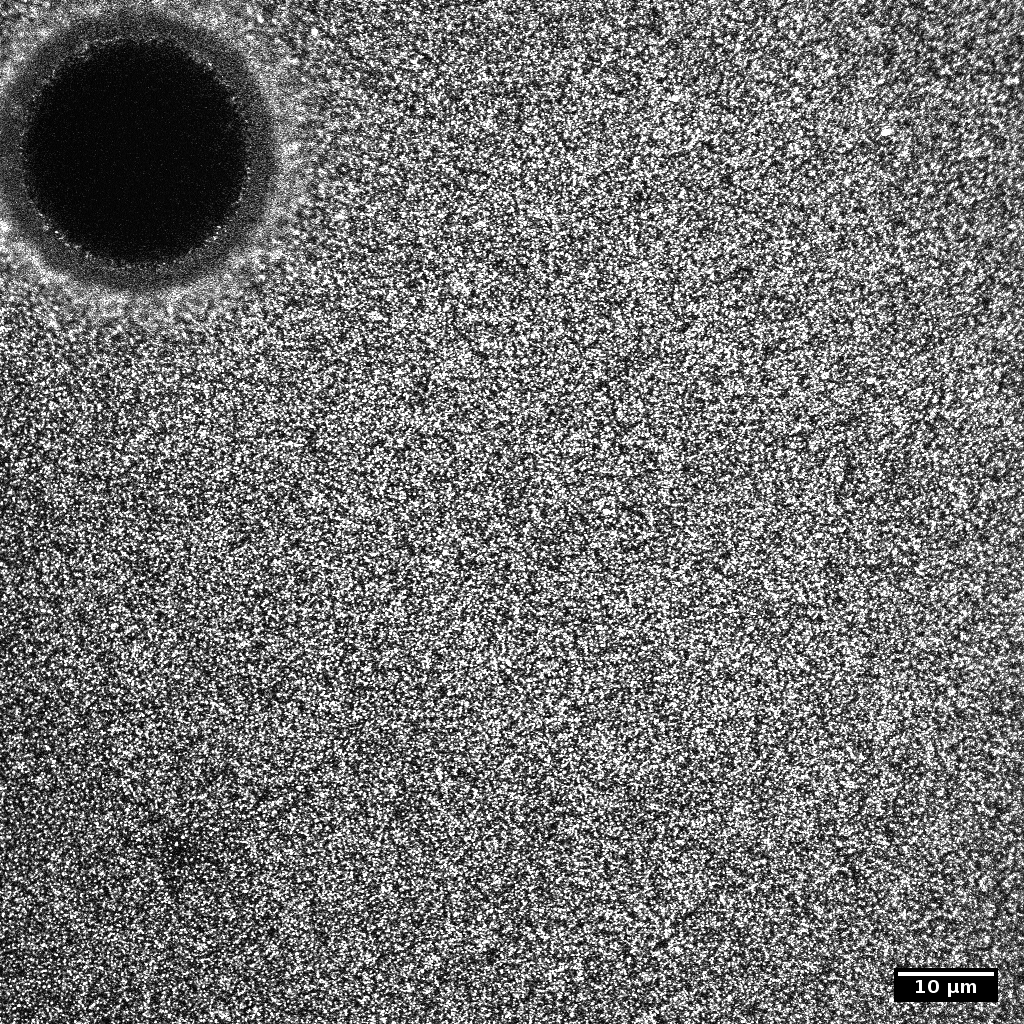
\includegraphics[width=.75\linewidth]{Chapters/Figures/190215_g91_glass_sphere011_surface.png}
	\caption[The surface plane of a silica bead in silcone]{The surface plane of a silica bead in Gelest 9:1 Silicone (E = 7.3 kPa). Radius of sphere = 28.7 $\mu$m.}
	\label{fig:190215g91glasssphere011surface}
\end{figure}
The object resembling a black hole in the top-left corner is the silica sphere. Each small white dot represents a fluorescent bead; together they create a sea of stars that outline the surface plane and the silica sphere. Figure \ref{fig:190215g91glasssphere011surface} is an example of the upper limit of bead coverage density. Any higher concentration of fluorescent beads could result in a difficulty in light bleeding. Note, the sphere is in the top corner of the image to provide maximum information about the leveling of the surface plane. We assume that the surface effects are symmetrical for zero applied strain and equibiaxial strain. Thus, it is more important to gather information in one direction to properly level the surface plane to determine the depth into which the sphere sinks. 

For each sphere, we take a stack of 50-100 images, depending on the size of the sphere. Table \ref{fig:sphere011cascade} shows several vertical slices from the bottom of the sphere to just above the surface of the substrate.

\begin{table}[h!]
	\begin{tabular}{ccc}
		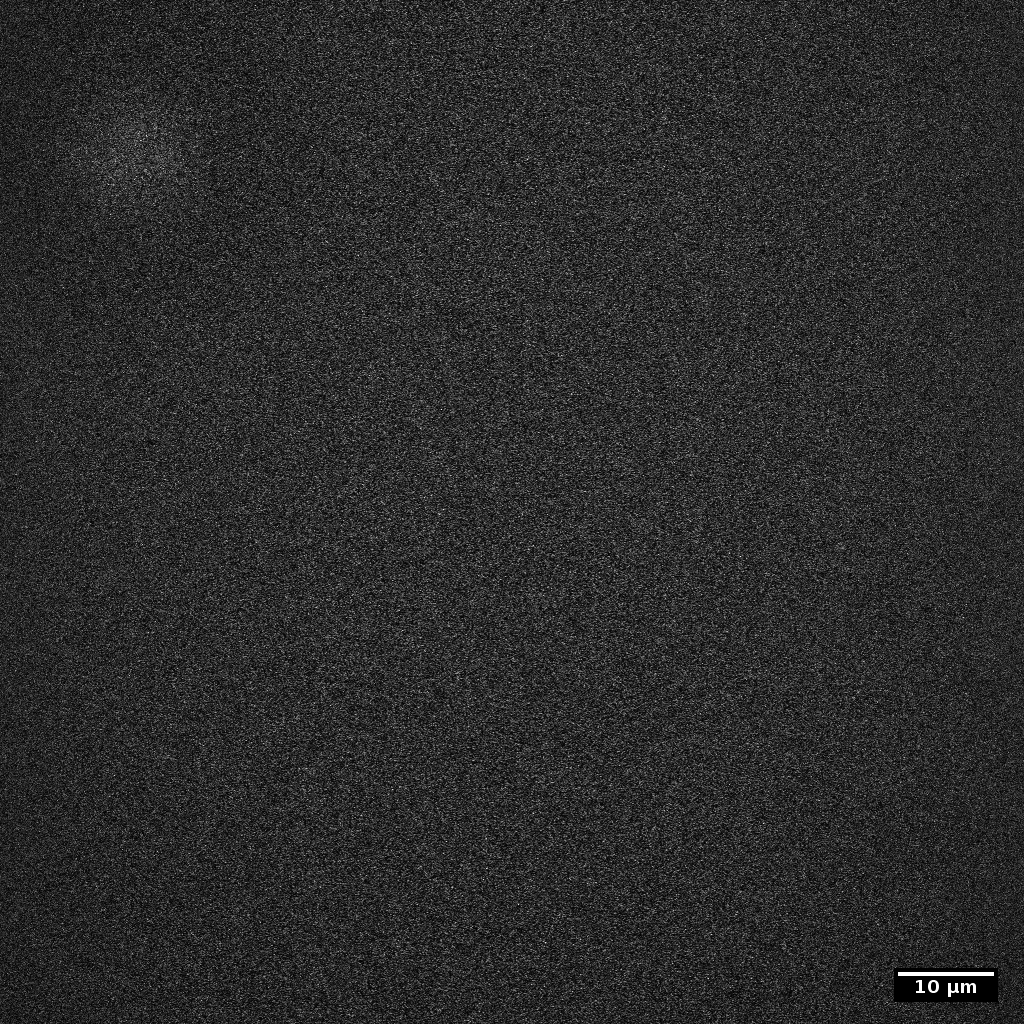
\includegraphics[width= .33\linewidth]{Chapters/Figures/190215_g91_glass_sphere011_cascade1.png} & 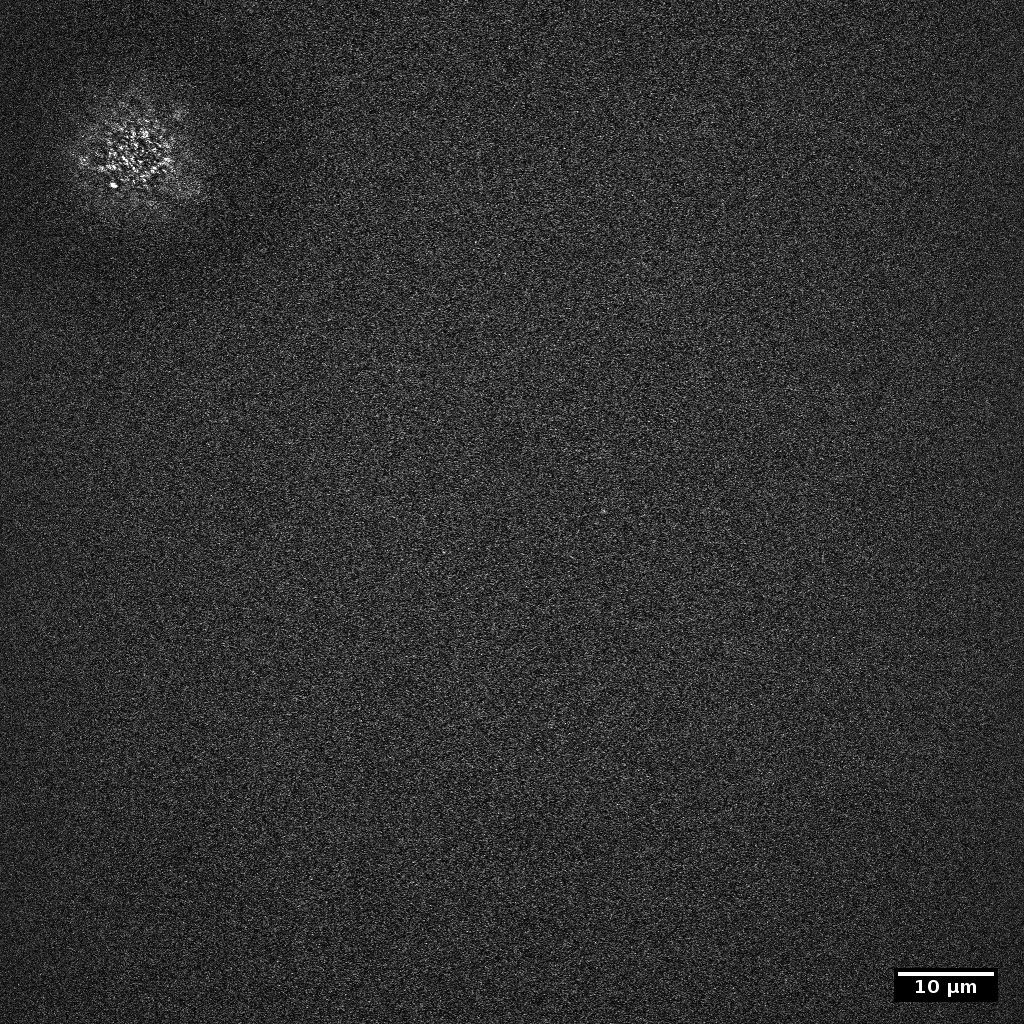
\includegraphics[width= .33\linewidth]{Chapters/Figures/190215_g91_glass_sphere011_cascade2.png} & 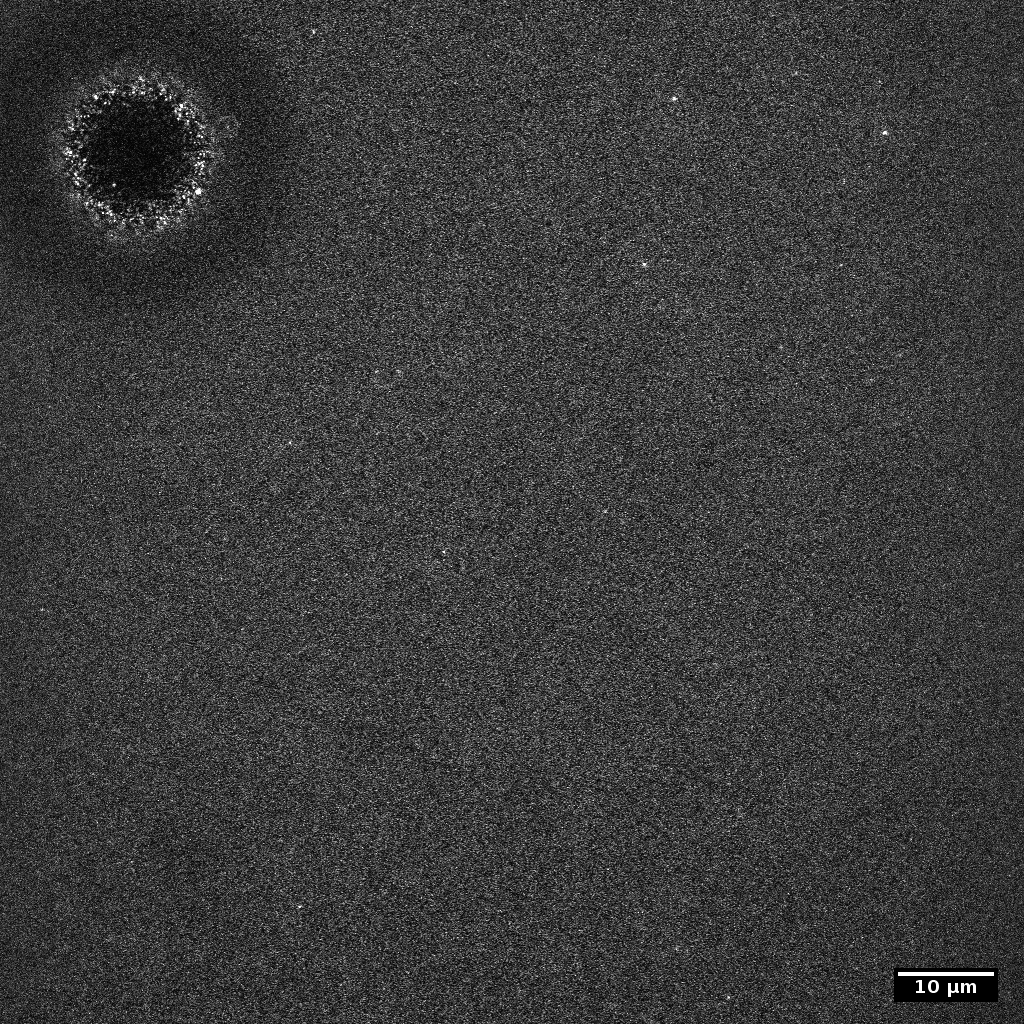
\includegraphics[width= .33\linewidth]{Chapters/Figures/190215_g91_glass_sphere011_cascade3.png} 
		\\
		a) & b) & c) \\
		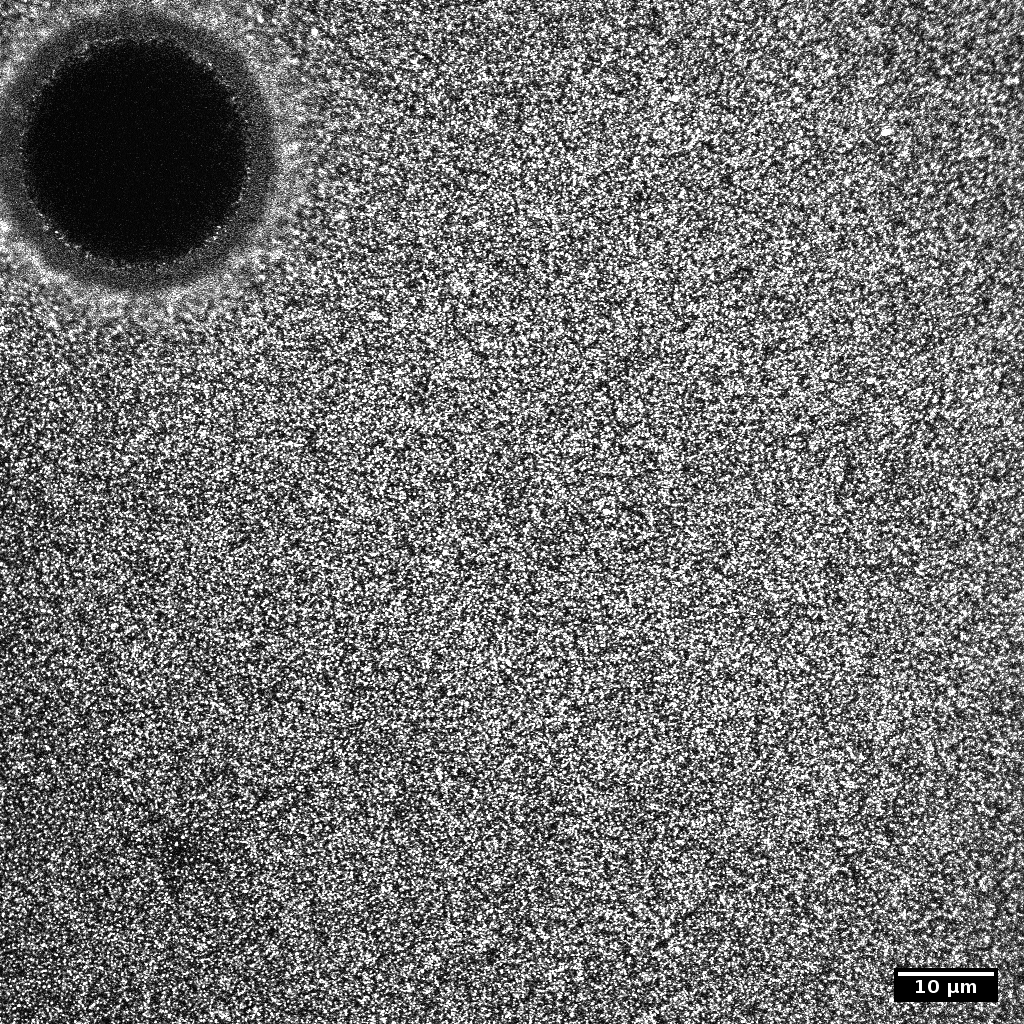
\includegraphics[width= .33\linewidth]{Chapters/Figures/190215_g91_glass_sphere011_cascade4.png} & 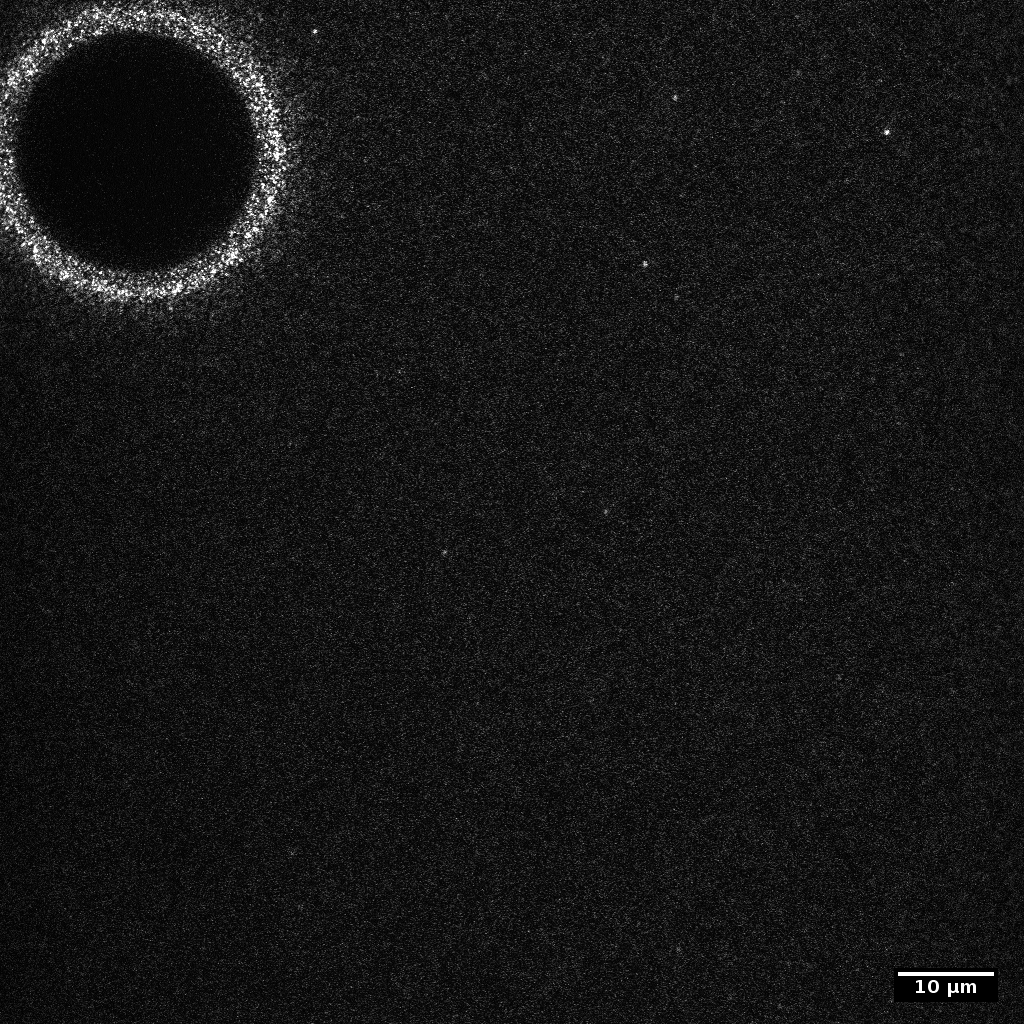
\includegraphics[width= .33\linewidth]{Chapters/Figures/190215_g91_glass_sphere011_cascade5.png} & 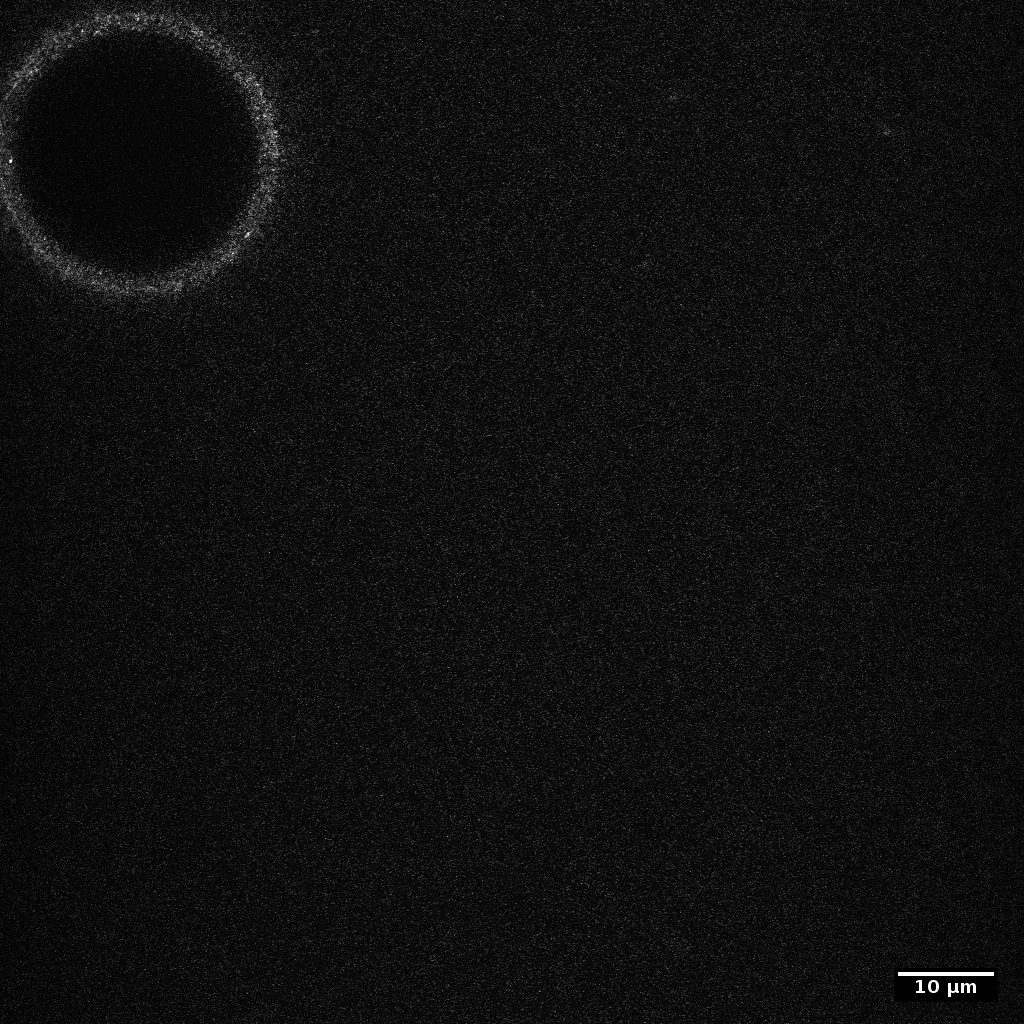
\includegraphics[width= .33\linewidth]{Chapters/Figures/190215_g91_glass_sphere011_cascade6.png}
		\\
		d) & e) & f) 
	\end{tabular}
	\caption[Vertical path through image stack]{Images a-f display the x-y plane of the same sample traversing vertically from below the silica sphere to above the surface plane. The scale bar in the bottom right corners represent 10 $\mu$m.} 
	\label{fig:sphere011cascade}
\end{table}


\section{Image Analysis}
In the following section, we will step through the process of analyzing a single sphere. Recall that in order to determine the surface stress and adhesion energy, we must fit equation \ref{THEeqn} to the depth vs. radius measurements for a collection of spheres.  

\subsection{Particle Location}
We use a MATLAB program to locate the fluorescent beads in each 3D raw image stack. This is plotted in Figure \ref{fig:particlelocatednormalized} for the same adhered sphere as in Figures \ref{fig:190215g91glasssphere011surface} and \ref{fig:sphere011cascade}. The flat orange plane of points is the surface, and the dark blue are the fluorescent beads pushed underneath the microsphere as it sinks into the substrate. It is easy to see the outline of the microsphere, and we can use this information to determine d and R for the sphere. 
Figure \ref{fig:particlelocatedstretched} shows the same sphere but stretched in the vertical axis to see the fluorescent bead density towards the bottom of the sphere. 
\begin{figure}[h]
	\centering
	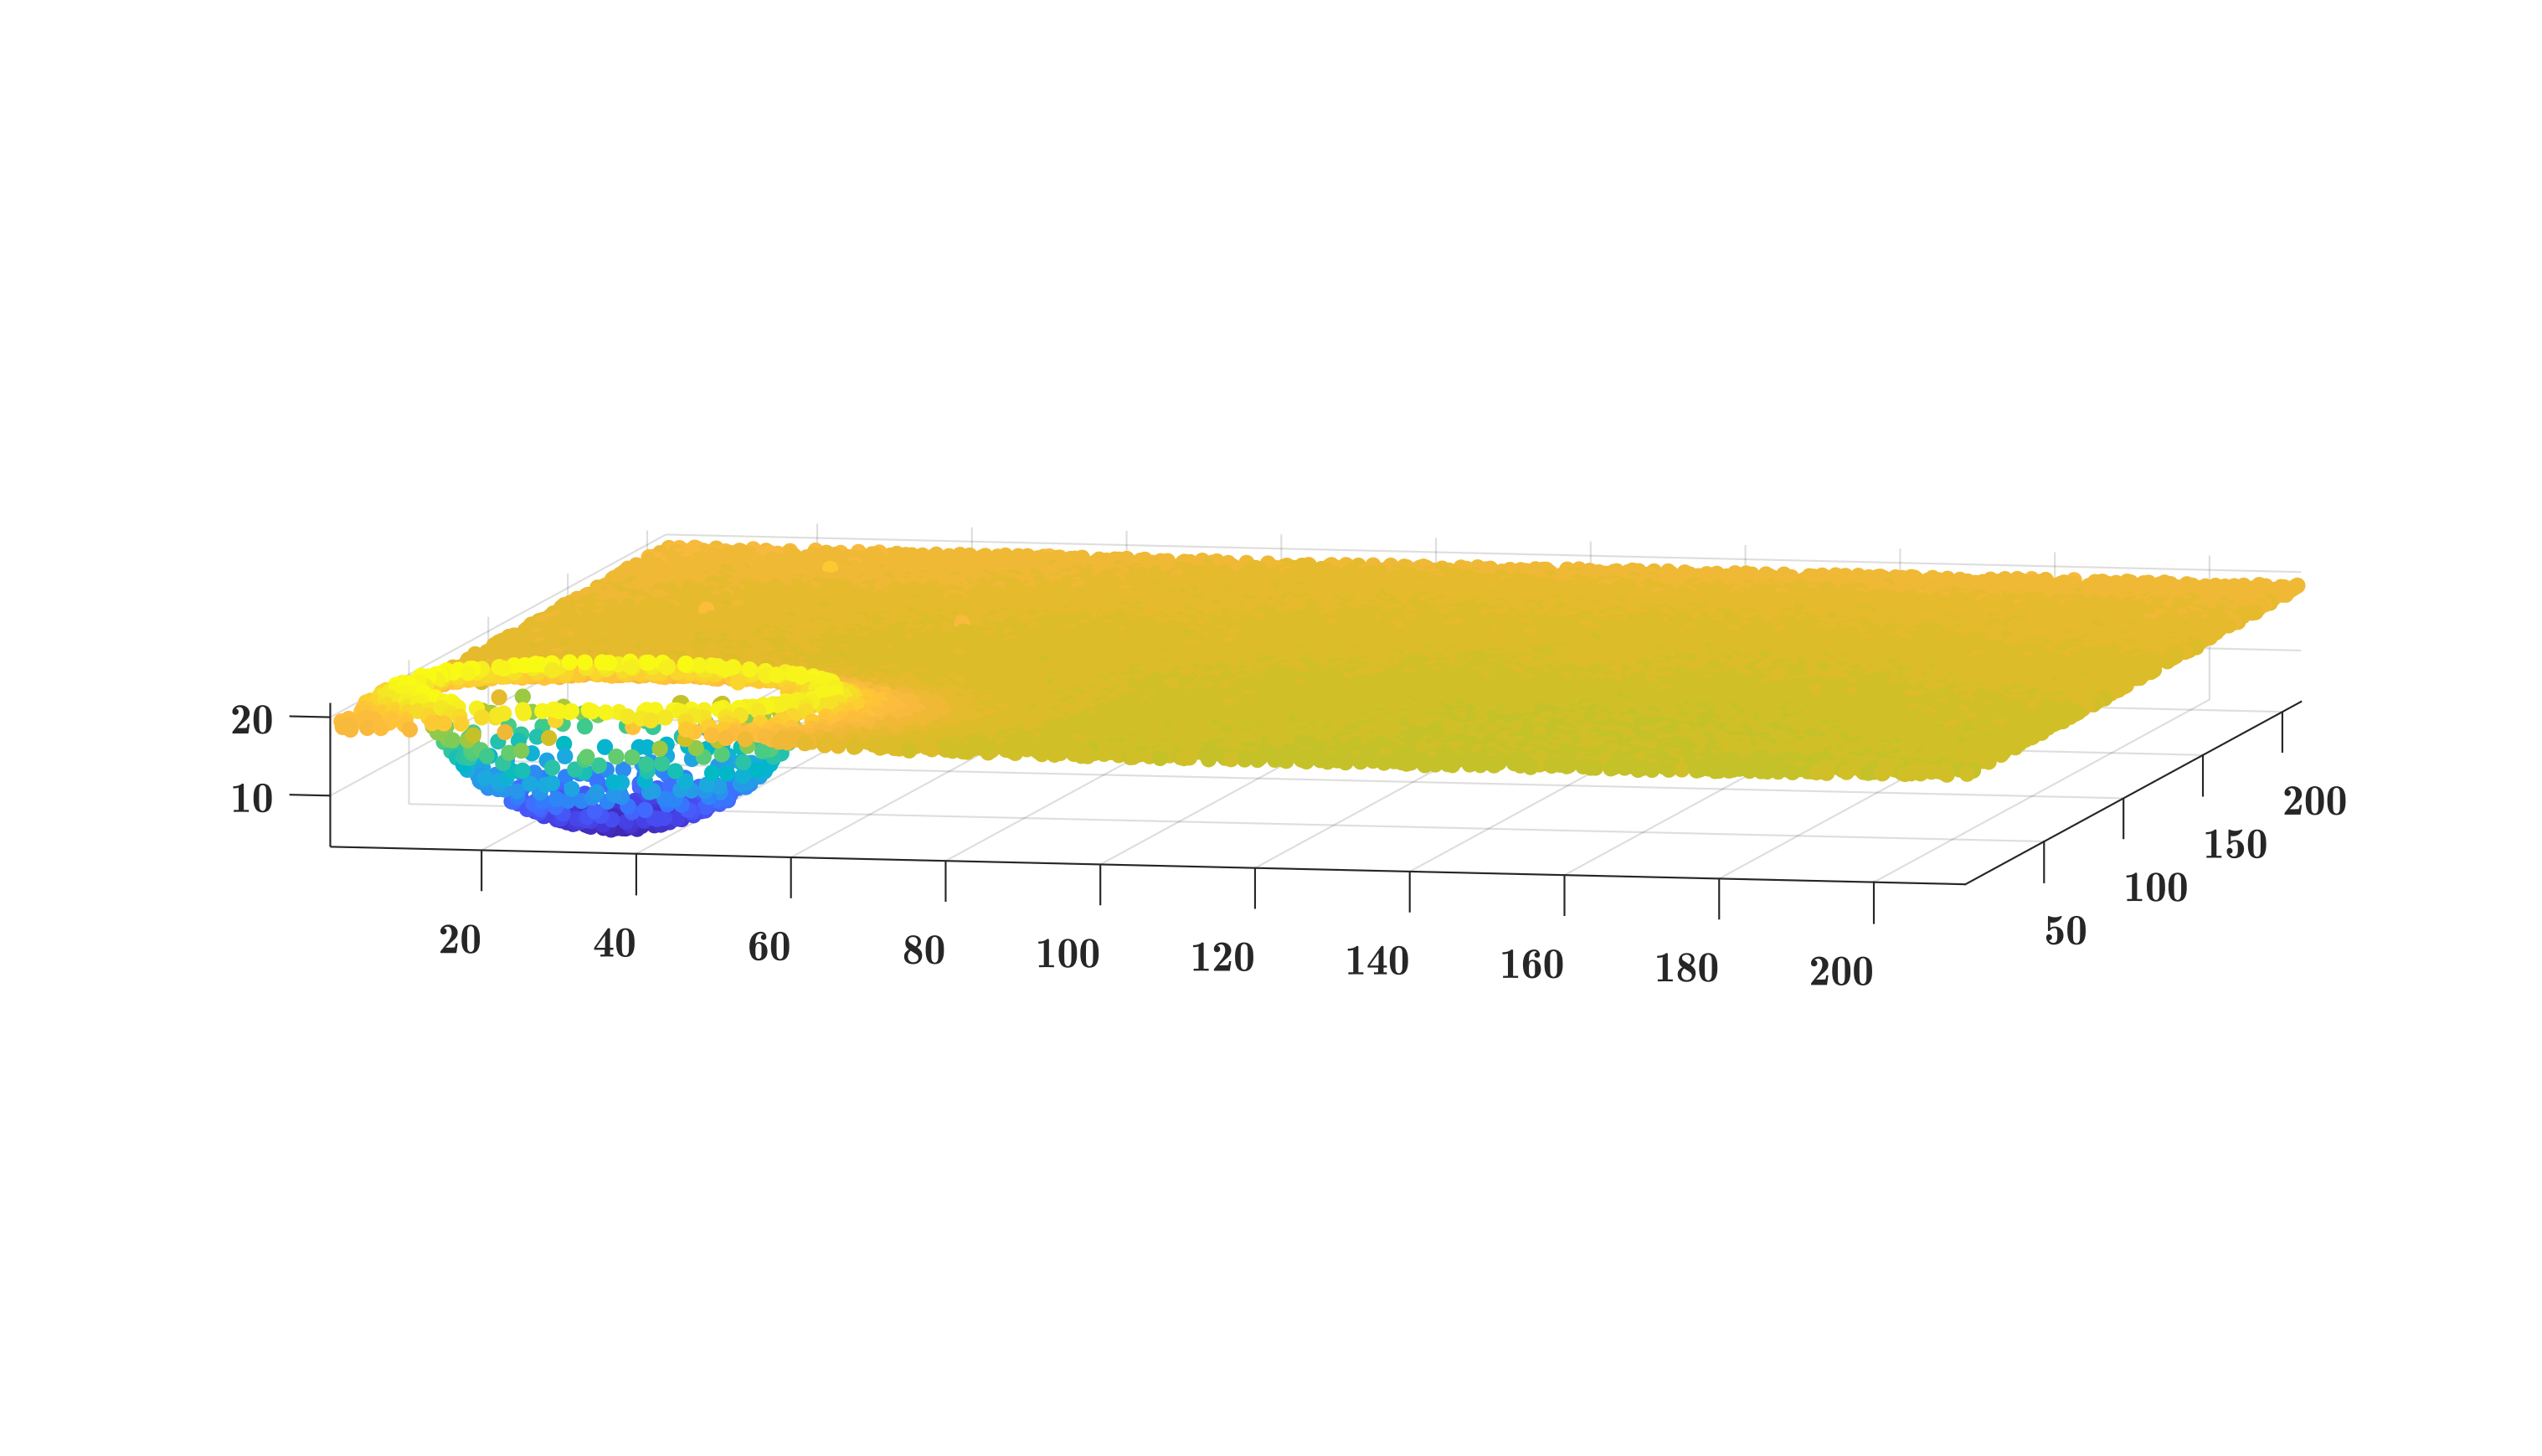
\includegraphics[width=\linewidth]{Chapters/Figures/sphere011_ia/particle_located_normalized}
	\caption[Particle Located: Normalized-Axes]{Using MATLAB sotware, we can locate each of the fluorescent beads in a given image stack. Here, we've plotted the located beads for the same sphere as in Figure \ref{fig:190215g91glasssphere011surface} and \ref{fig:sphere011cascade}. The dense blanket of orange points represents the surface of the substrate, and the blue points are the fluorescent beads pushed beneath the silica sphere during indentation.}
	\label{fig:particlelocatednormalized}
\end{figure}


\begin{figure}[h!]
	\centering
	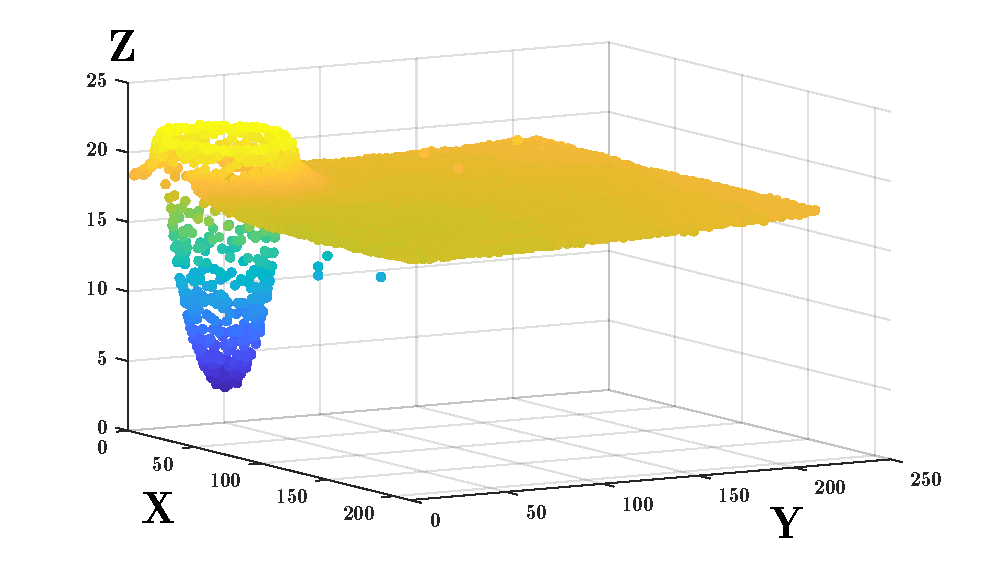
\includegraphics[width=\linewidth]{Chapters/Figures/sphere011_ia/particle_located_stretched}
	\caption[Particle Located: Stretched-Axes]{Fluorescent bead location for the same sphere as Fig.  \ref{fig:particlelocatednormalized} with vertical axis stretched to showcase the bead density under the bottom of the sphere.}
	\label{fig:particlelocatedstretched}
\end{figure}

\begin{figure}[h]
	\centering
	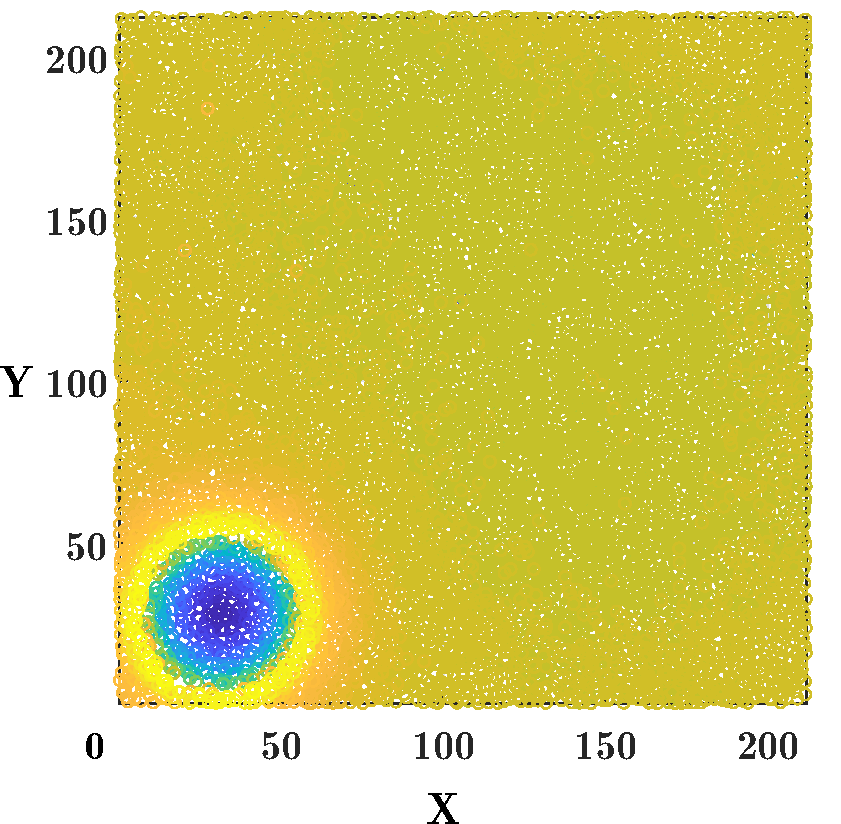
\includegraphics[width=.8\linewidth]{Chapters/Figures/sphere011_ia/particle_located_top_view}
	\caption[Particle Located: Top View]{Here is the top view of the same sphere as in the previous figures. This allows us locate the center of the base of the sphere. From this we can construct a side profile (\ref{fig:sidecollapsed})}
	\label{fig:particlelocatedtopview}
\end{figure}
\subsection{Depth and Radius Determination}
After locating all the fluorescent beads and reconstructing our raw image in a useful format, we can then use this information to extract the depth and the radius of the sphere. To accomplish this, we first determine the center of the sphere from the top (x-y plane) and collapse the surface profile azimuthally about the sphere's center position. Figure \ref{fig:sidecollapsed} depicts the x-z plane as a cross-section through center of the sphere. We only need half of the sphere's profile to fit a circle. This ensures we have a large field of view to properly level and determine the substrate's surface. Figure \ref{fig:sidecollapsedzoomed} provides a zoomed in view of Fig. \ref{fig:sidecollapsed} to better indicate the resolution to which we try to fit a circle. Note the abrupt cut off around o$r = 26$ $ \mu$m and how the substrate is lifted up above the zero-plane due to adhesion. Also notice the flatness on of the substrate between $r= 26-29$ $\mu $m. Not all sample have this flat ridge; many sphere lift the substrate to a point which the immediately slopes downward back to the zero-plane. This behavior depends slightly on the sphere size, but it is mainly a reflection of the amount of phase-separation induced. This is a property of the each silicone which depends on the environmental conditions. 


\begin{figure}[h!]
	\centering
	\large \textbf{No Applied Strain (On Glass): Large Sphere}\\ \vspace{.4 em}
	\large \textbf{Gelest 9:1 (E=6.3kPa)}
	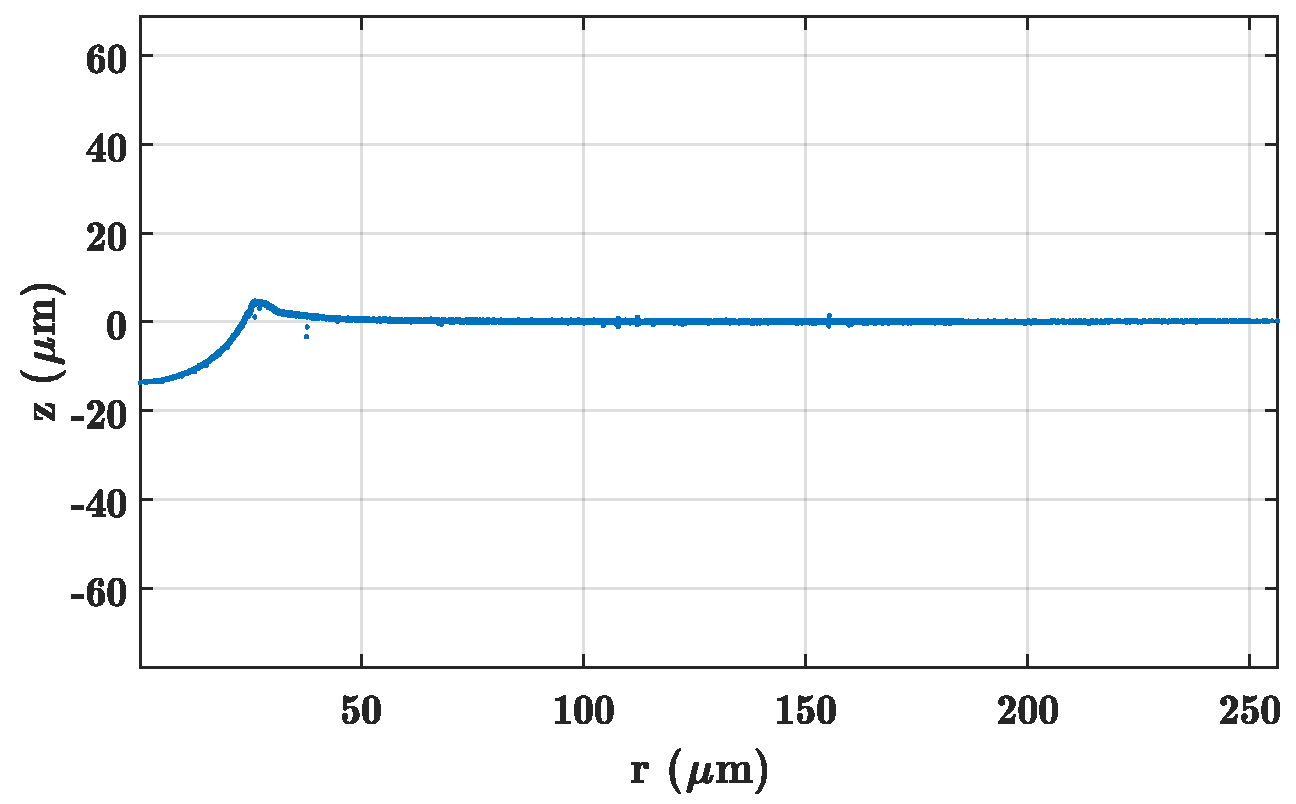
\includegraphics[width=\linewidth]{Chapters/Figures/sphere011_ia/side_collapsed}
	\caption[Collapsed Side Profile]{TThe full surface profile, collapsed azimuthally. From this, the region conforming to the adhered sphere is clearly visible}
	\label{fig:sidecollapsed}
\end{figure}
\begin{figure}[h!]
	\centering
	\large \textbf{No Applied Strain (On Glass): Large Sphere}\\ \vspace{.4 em}
	\large \textbf{Gelest 9:1 (E=6.3kPa)}
	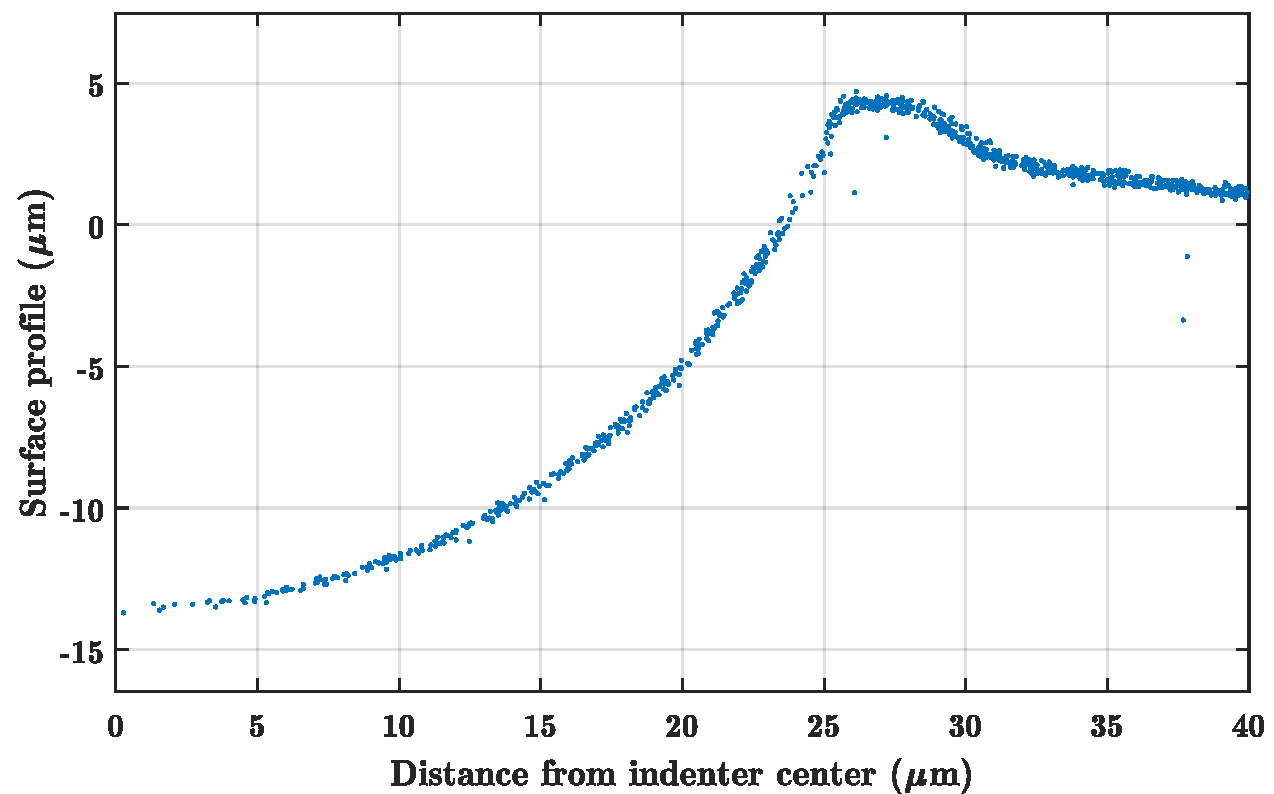
\includegraphics[width=\linewidth]{Chapters/Figures/sphere011_ia/side_collapsed_zoomed}
	\caption[Collapsed Side Profile: Zoomed]{This is a zoomed-in version of Figure \ref{fig:sidecollapsed}. It is useful to zoom in and see the the quality of the collapse. A dense collapse leads to a smaller margin of error in fitting a circle to the profile (See Fig. \ref{fig:circlefit}).}
	\label{fig:sidecollapsedzoomed}
\end{figure}
\begin{figure}[h!]
	\centering
	\large \textbf{No Applied Strain (On Glass): Large Sphere}\\ \vspace{.4em}
	\large \textbf{Gelest 9:1 (E=6.3kPa)}
	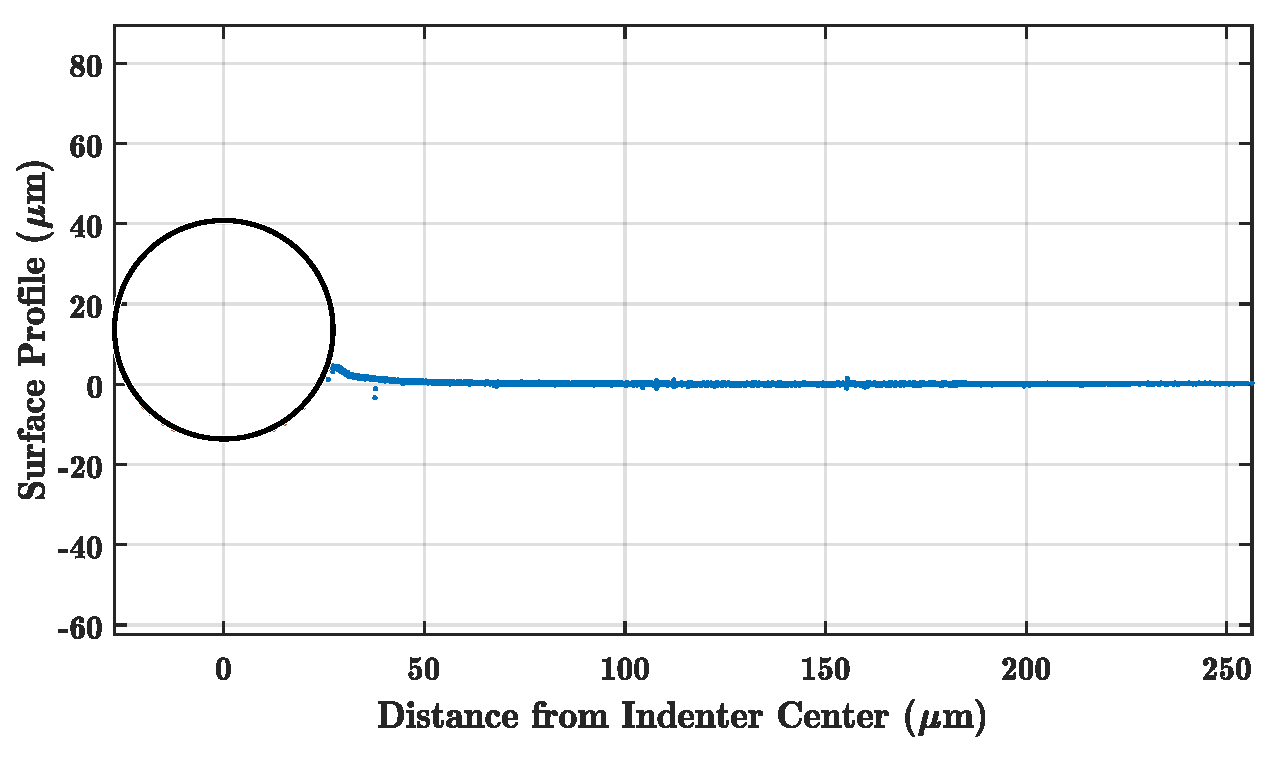
\includegraphics[width=\linewidth]{Chapters/Figures/sphere011_ia/circle_fit}
	\caption[Circle Fit]{This is figure \ref{fig:sidecollapsed}, only with a circle fitted to the indentation sphere. Notice how the surface plane is completely flat and centered at a depth of 0.}
	\label{fig:circlefit}
\end{figure}


\begin{figure}[h!]
	\centering
	{\large \textbf{No Applied Strain (On Glass): Large Sphere}}\\ \vspace{.4 em}
	{\large \textbf{Gelest 9:1 (E=6.3kPa)}}
	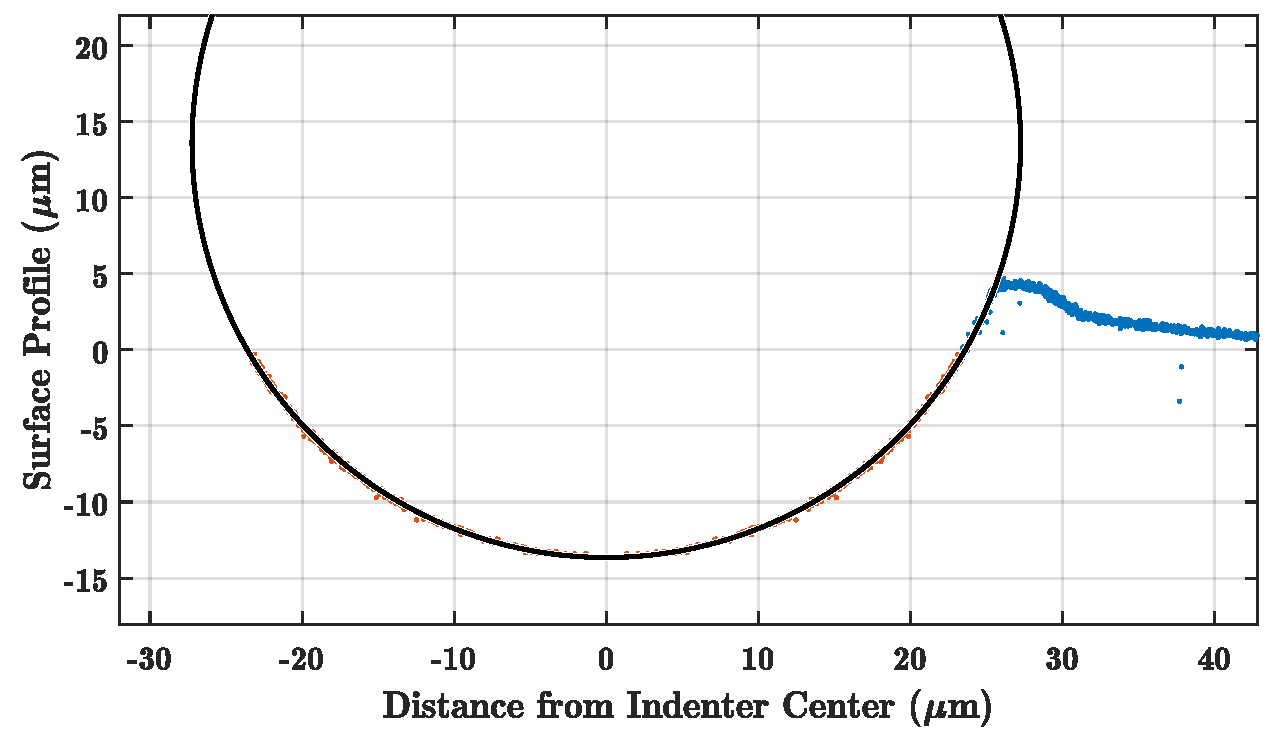
\includegraphics[width=\linewidth]{Chapters/Figures/sphere011_ia/circle_fit_zoomed}
	\caption[Circle Fit Zoomed]{This is simply a zoomed in version of Figure \ref{fig:circlefit}. The orange dots are the data points being used to fit the circle. Notice how the sphere fits nicely in the indentation all the way up to the cusp, past the points being used for the fit.}
	\label{fig:circlefitzoomed}
\end{figure}

It is important to be careful with the circle-fits in the case where the sphere is small enough to sink into the substrate with a depth $ d > r $. In these instances, the the side profile is non-continuous, and we only fit the sphere to the bottom portion of the profile before the break. An example of one of these sphere is shown in figures \ref{fig:smallsphere017190404dcglass} and \ref{fig:smallsphere017ciclefitspheredc}.
\begin{figure}[h!]
	\centering
	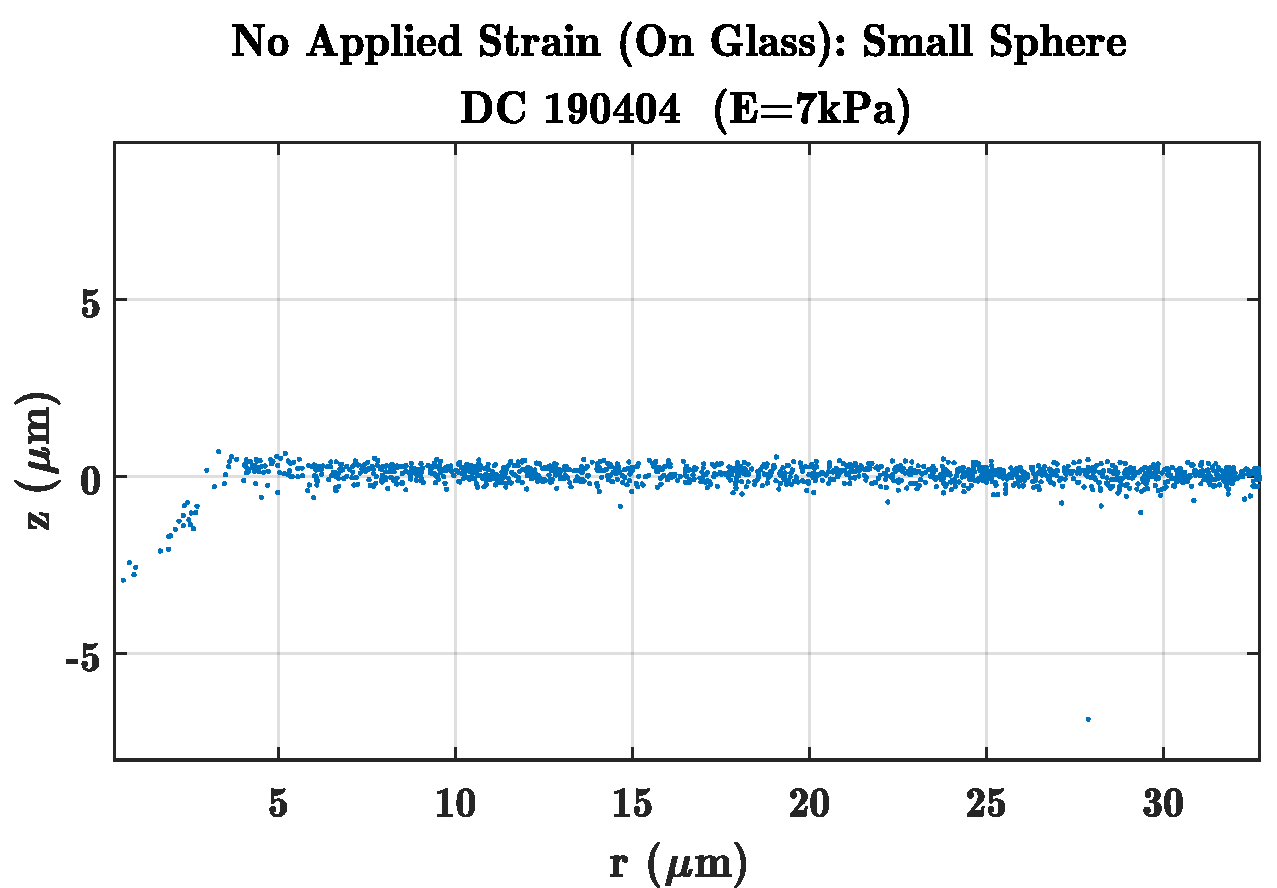
\includegraphics[width=\linewidth]{Chapters/Figures/smallsphere017_190404_DC_glass}
	\caption[Small Sphere Side Profile]{The collapase side profile for small spheres has fewer fluorescent tracer particles to outline there sphere. There is often a cutoff if the sphere sinks in deeper than its ``waist.''}
	\label{fig:smallsphere017190404dcglass}
\end{figure}
\begin{figure}[h!]
	\centering
	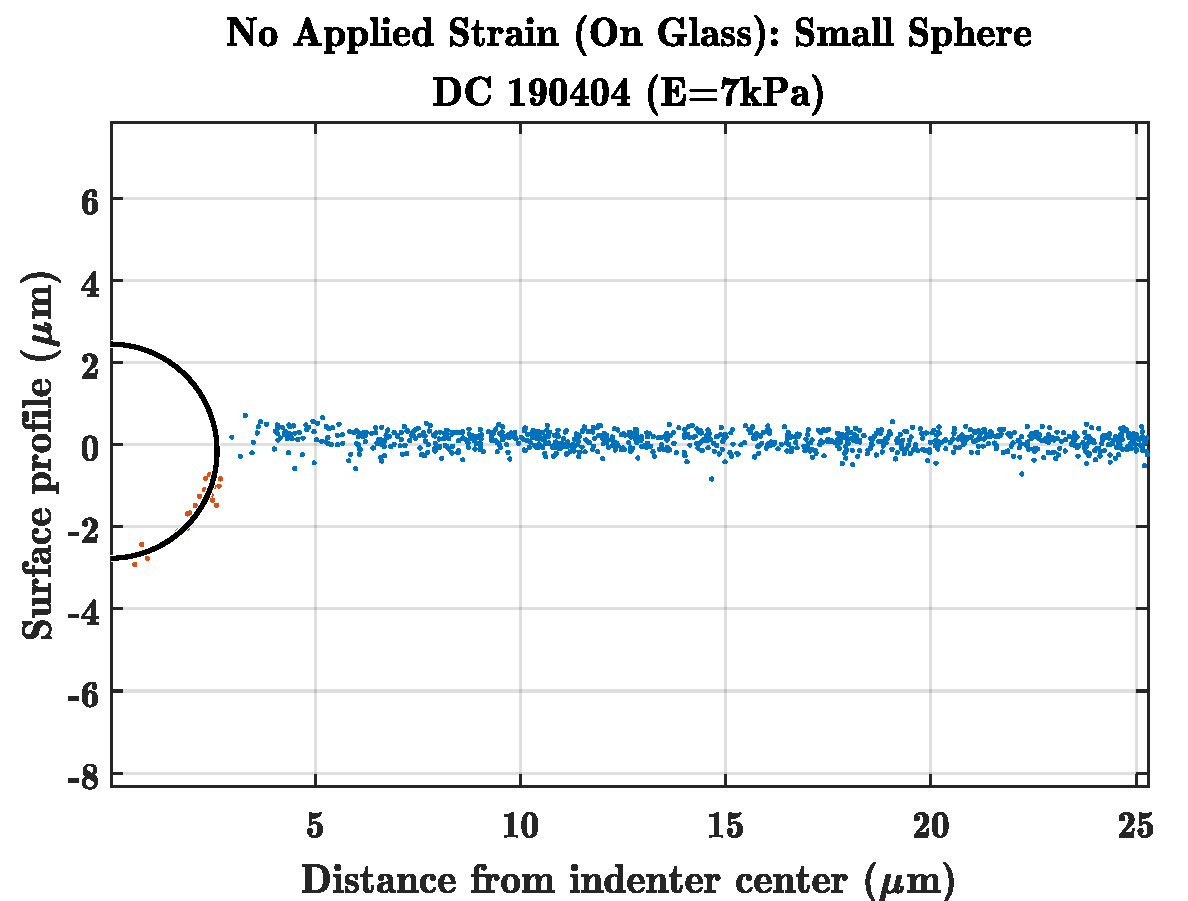
\includegraphics[width=\linewidth]{Chapters/Figures/smallsphere017_cicle_fitsphere_DC}
	\caption[Small Sphere Circle Fit]{For a small sphere where d>r, there is generally a break in the sphere outline. For these circle fits, only the fluorescent beads up to the break are taken into account for the fit.}
	\label{fig:smallsphere017ciclefitspheredc}
\end{figure}




After fitting the circle to the substrate's side profile, we can extract the depth versus radius. The radius of the sphere equals the radius of the circle, and the depth is the lowest point of the circle in the z-plane, which we center at $ x=0 $ in Figures \ref{fig:circlefit} and \ref{fig:circlefitzoomed}.  
\begin{figure}
	\centering
	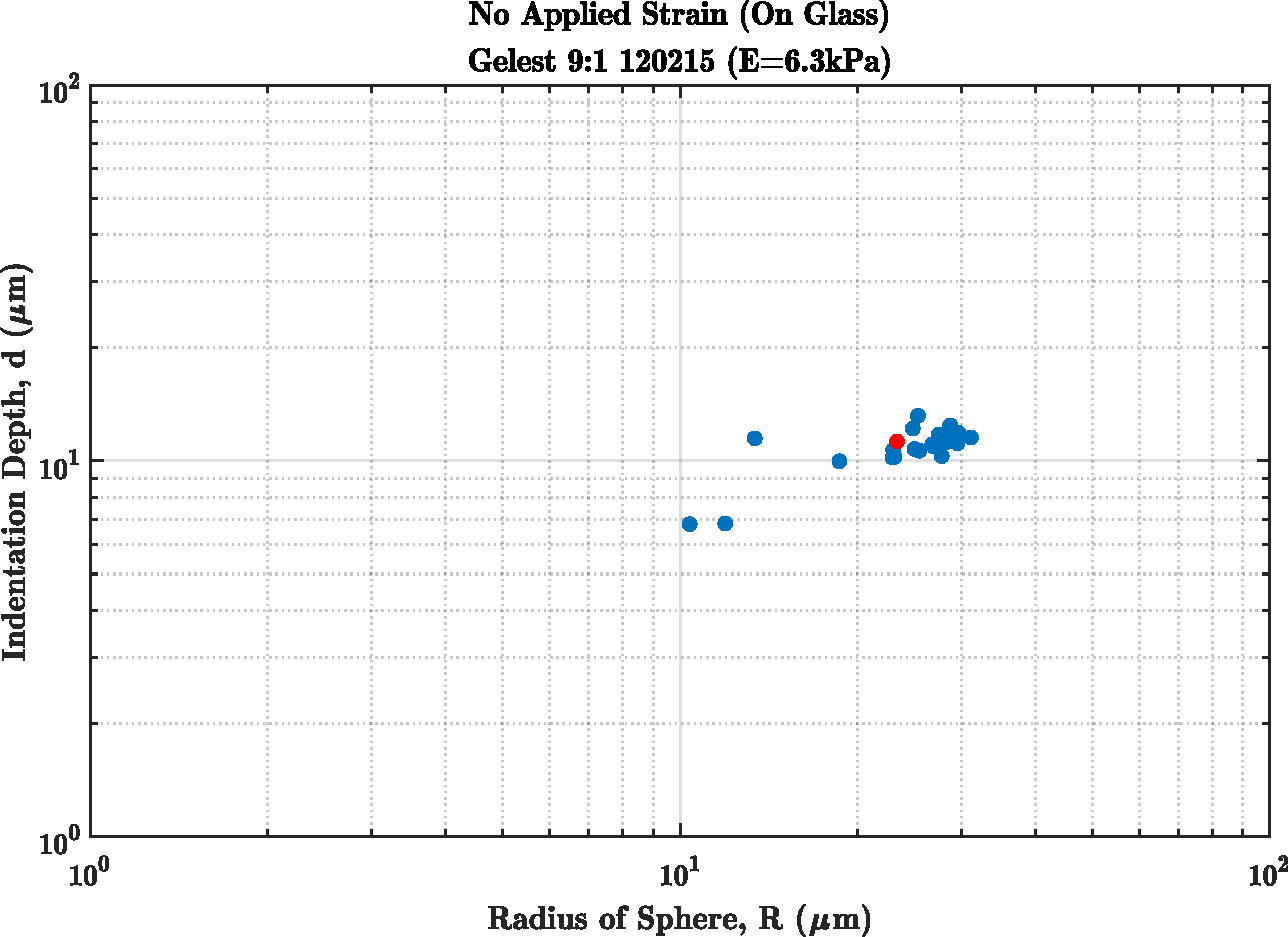
\includegraphics[width=\linewidth]{Chapters/Figures/d_vs_R_190215_sphere11highlight}
	\caption[Depth vs. Radius Example]{Here, we plot the spontaneous indentation depth vs. radius for a variety of sphere on a PDMS substrate. The red point indicates the same sphere that was examined in Figures \ref{fig:190215g91glasssphere011surface} - \ref{fig:circlefitzoomed}}
	\label{fig:dvsr190215sphere11highlight}
\end{figure}

%\begin{figure}
%	\centering
%	{\large \textbf{No Applied Strain (On Glass): Large Sphere}}\\ \vspace{.4em}
%	{\large \textbf{Gelest 9:1 (E=6.3kPa)}}
%	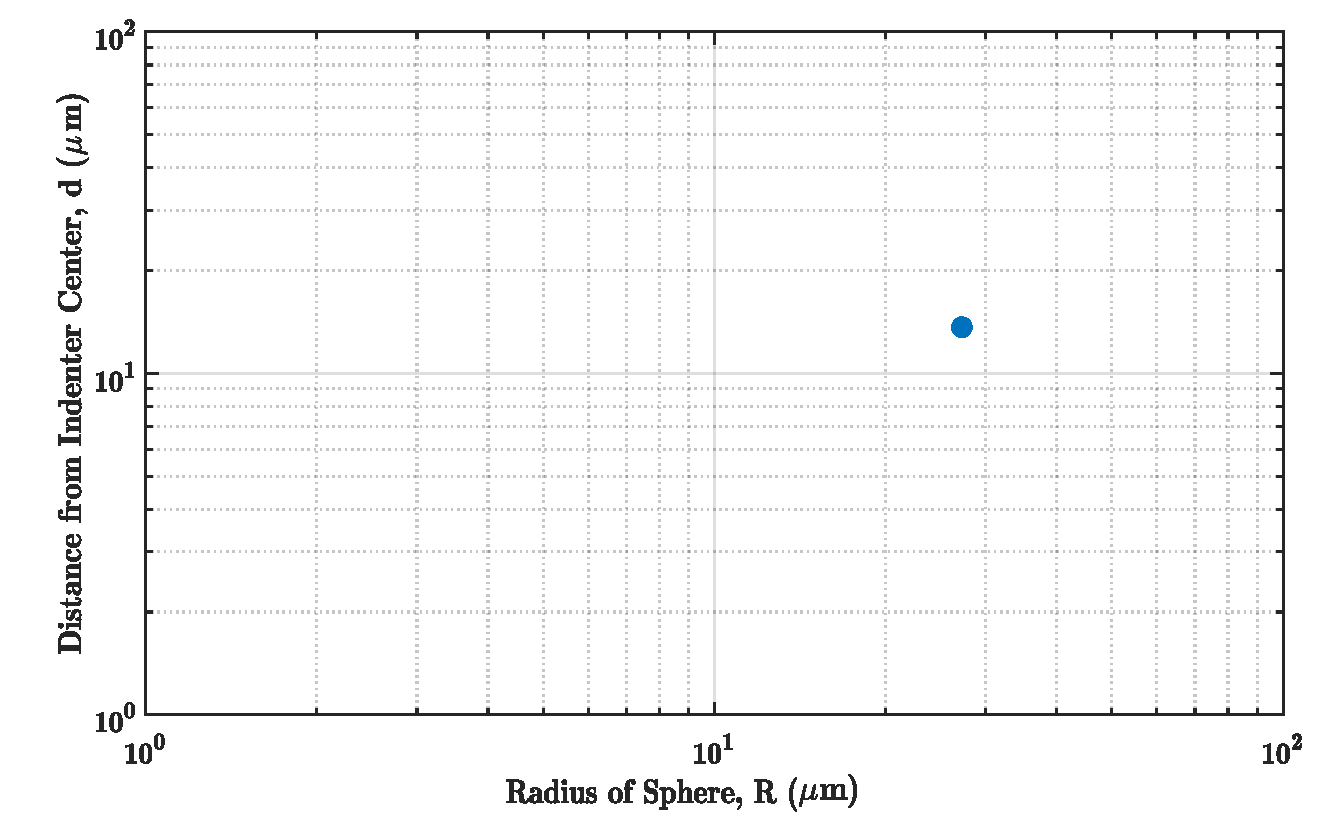
\includegraphics[width=\linewidth]{Chapters/Figures/sphere011_ia/single_d_vs_r}
%	\caption[D vs R plot]{All the above analysis leads to this single point, the depth, $ d $ vs. radius $ r $ for a given sphere. By repeating this process for many spheres of varying size, we can fill out the plot and fit equation \ref{THEeqn} to the points. Examples of these fits can be found in Chapter 4.}
%	\label{fig:singledvsr}
%\end{figure}
